La interacción con la interfaz es sencilla,
los botones tienen dos funcionalidades principales que son la de redirigir a otra página o la de realizar una acción.

Esta acción puede ser la de abrir un modal, como en el caso de la subasta de una carta o un menú desplegable, como en el caso del menú de usuario.

Los comportamientos más complejos de la interfaz son los de la subasta de una carta y la compra de un sobre de cartas.
Estos comportamientos se han diseñado de forma que sean intuitivos y fáciles de entender para el usuario.

A continuación, se mostrará un ejemplo de cada uno de estos comportamientos.

\subsubsection{Subasta de una carta}
En la \coloredUnderline{\hyperlink{fig:interfaz-subasta}{Figura \ref*{fig:interfaz-subasta}}} se muestra la vista del modal de crear una subasta.
En esta vista, el usuario puede seleccionar el precio de salida de la carta y el tiempo que durará la subasta.

\begin{figure}[H]
    \centering
    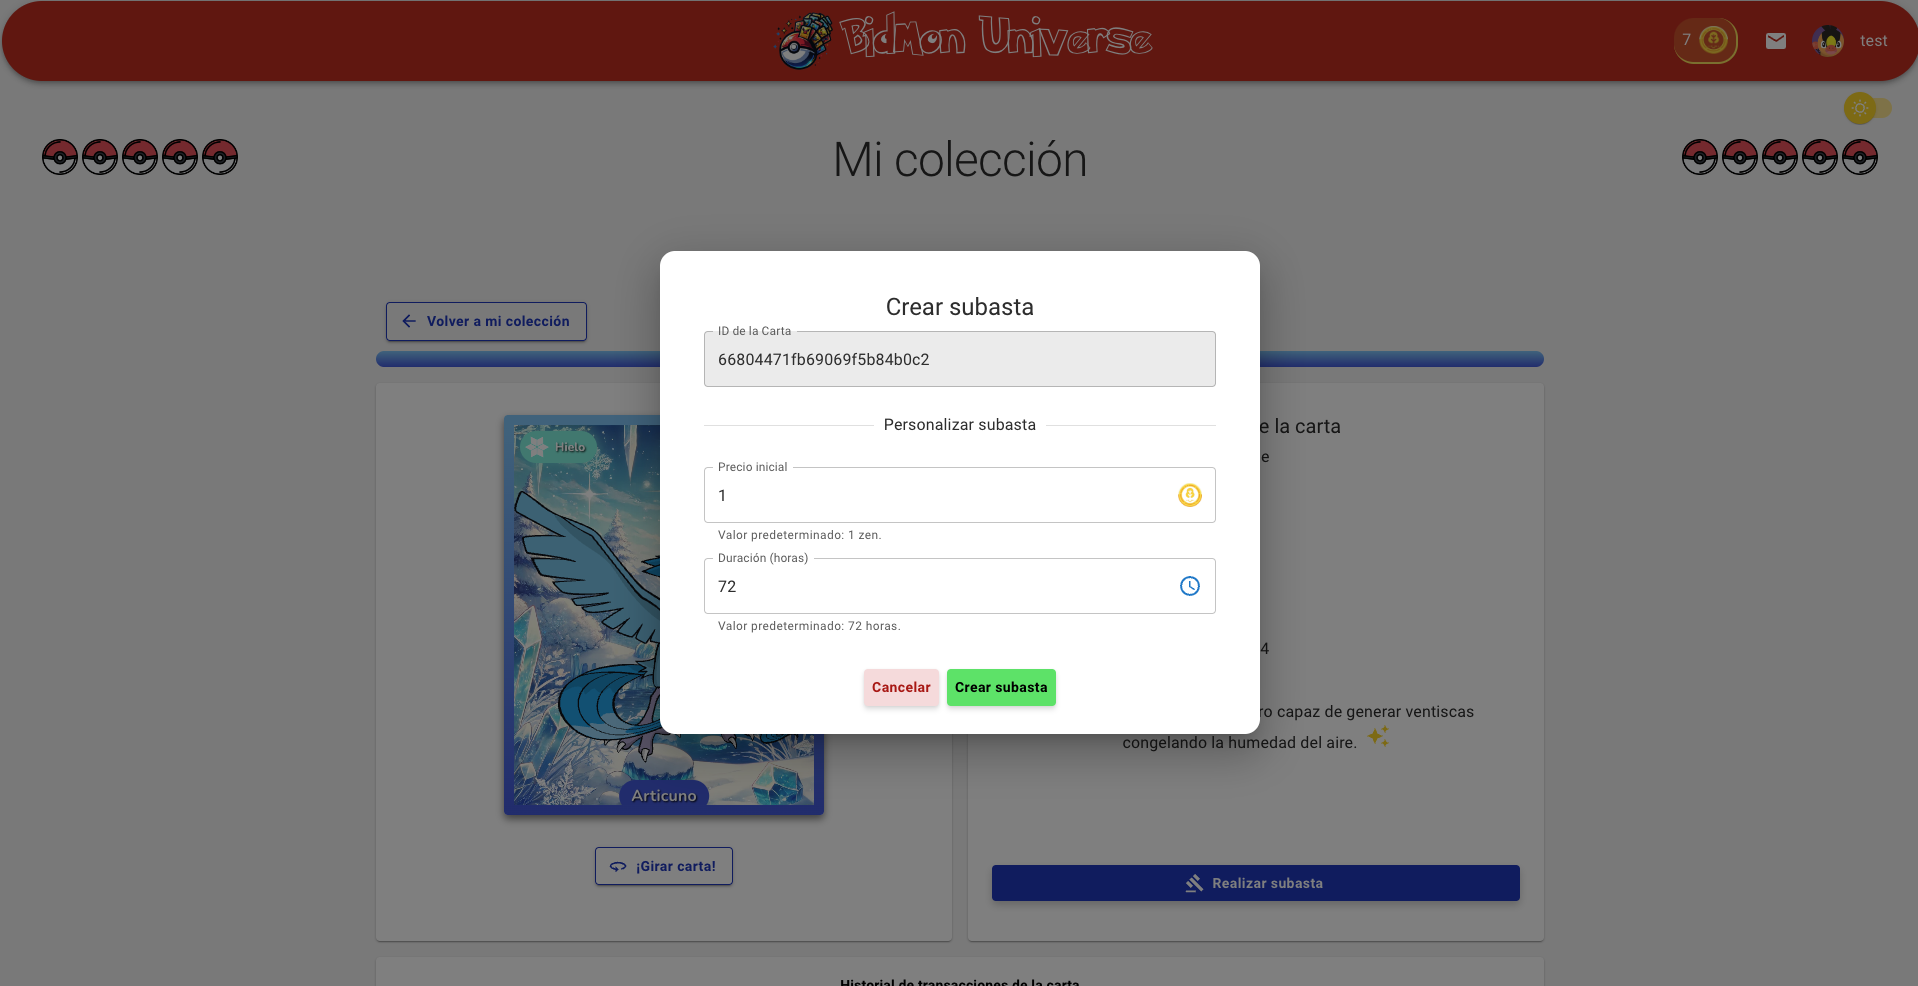
\includegraphics[width=0.8\textwidth]{figures/6-Analisis/6-Interfaz/interfaz/crear-subasta1.png}
    \caption{Modal de creación de subasta.}
    \hypertarget{fig:interfaz-subasta}{}
    \label{fig:interfaz-subasta}
\end{figure}

Una vez que el usuario ha rellenado los campos, puede pulsar el botón de \textit{Crear subasta} para confirmar la subasta.
Se le abrirá un modal de confirmación, en el que se le mostrará un resumen de la subasta y podrá confirmarla o cancelarla.

\begin{figure}[H]
    \centering
    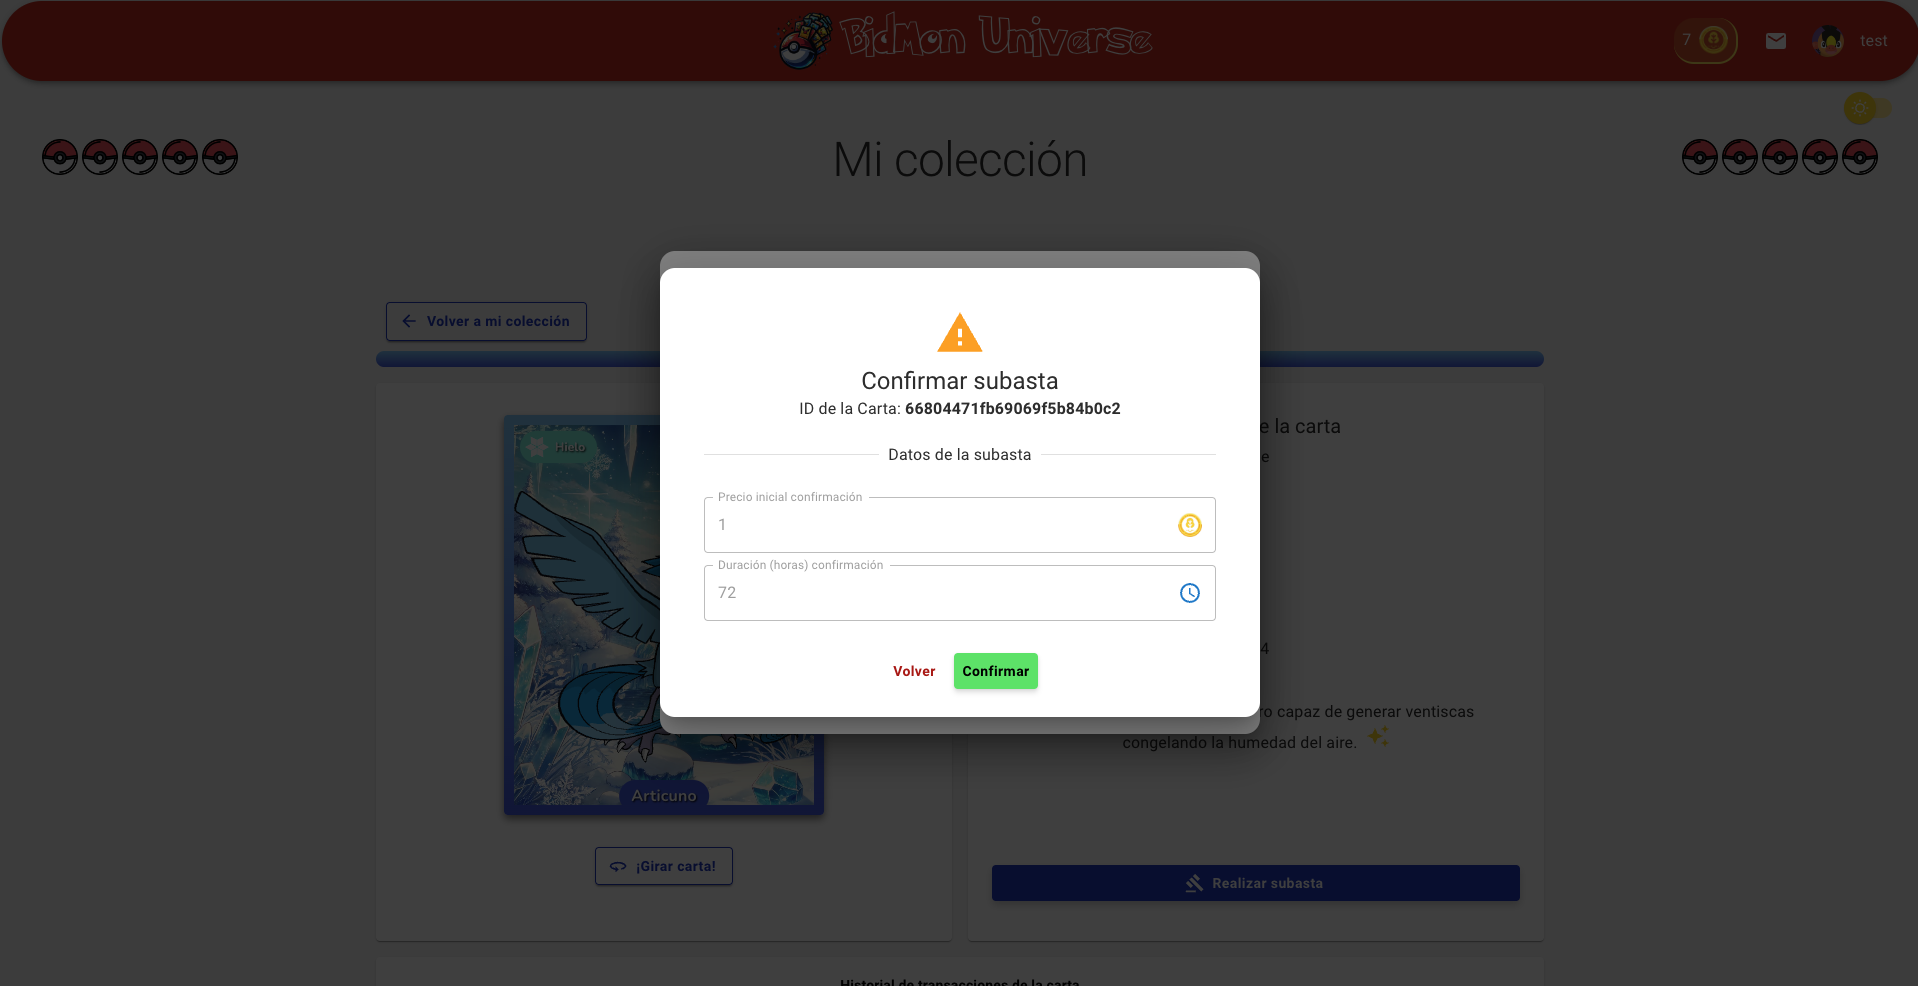
\includegraphics[width=0.8\textwidth]{figures/6-Analisis/6-Interfaz/interfaz/crear-subasta2.png}
    \caption{Modal de confirmación de subasta.}
    \label{fig:interfaz-subasta-alerta}
\end{figure}

Si confirma la subasta, se mostrará un mensaje de éxito, se cerrará el modal y desparecerá el botón de subastar reemplazándolo por una
alerta informativa de que la carta está en subasta.

\begin{figure}[H]
    \centering
    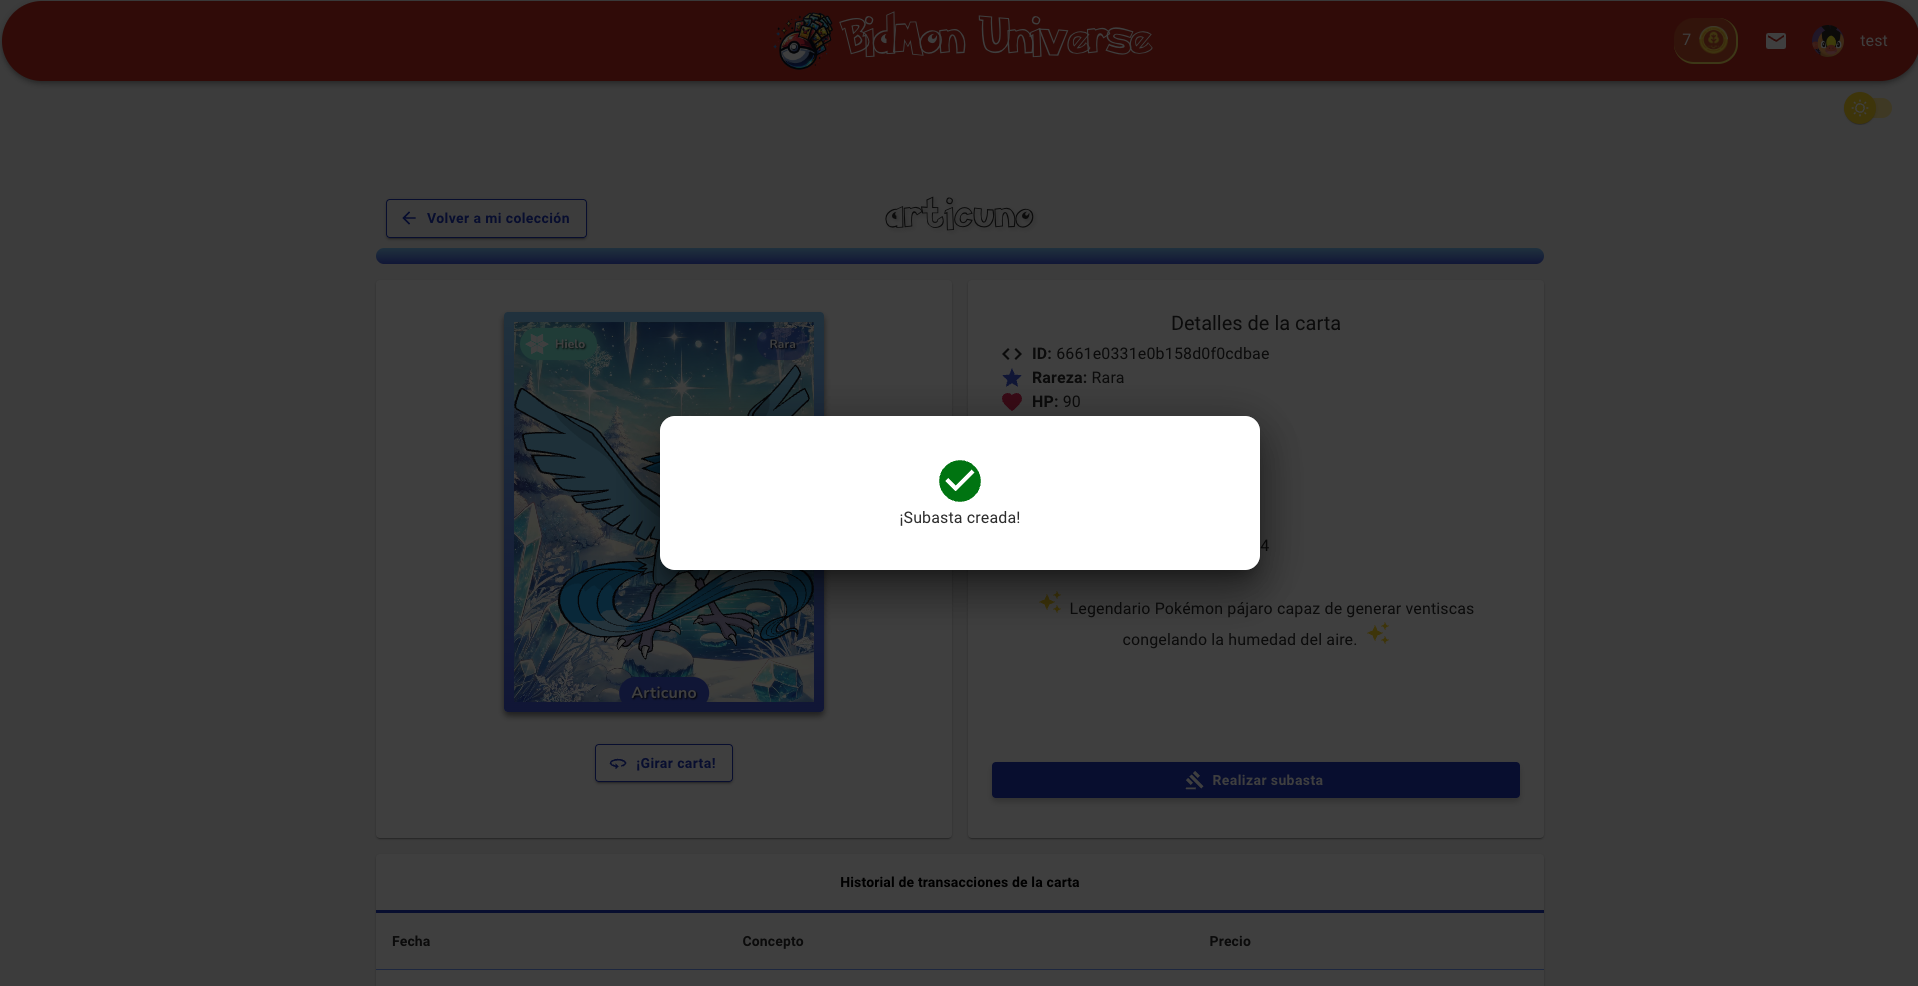
\includegraphics[width=0.8\textwidth]{figures/6-Analisis/6-Interfaz/interfaz/subasta_creada.png}
    \caption{Mensaje de éxito de creación de subasta.}
    \label{fig:interfaz-subasta-exito}
\end{figure}

\begin{figure}[H]
    \centering
    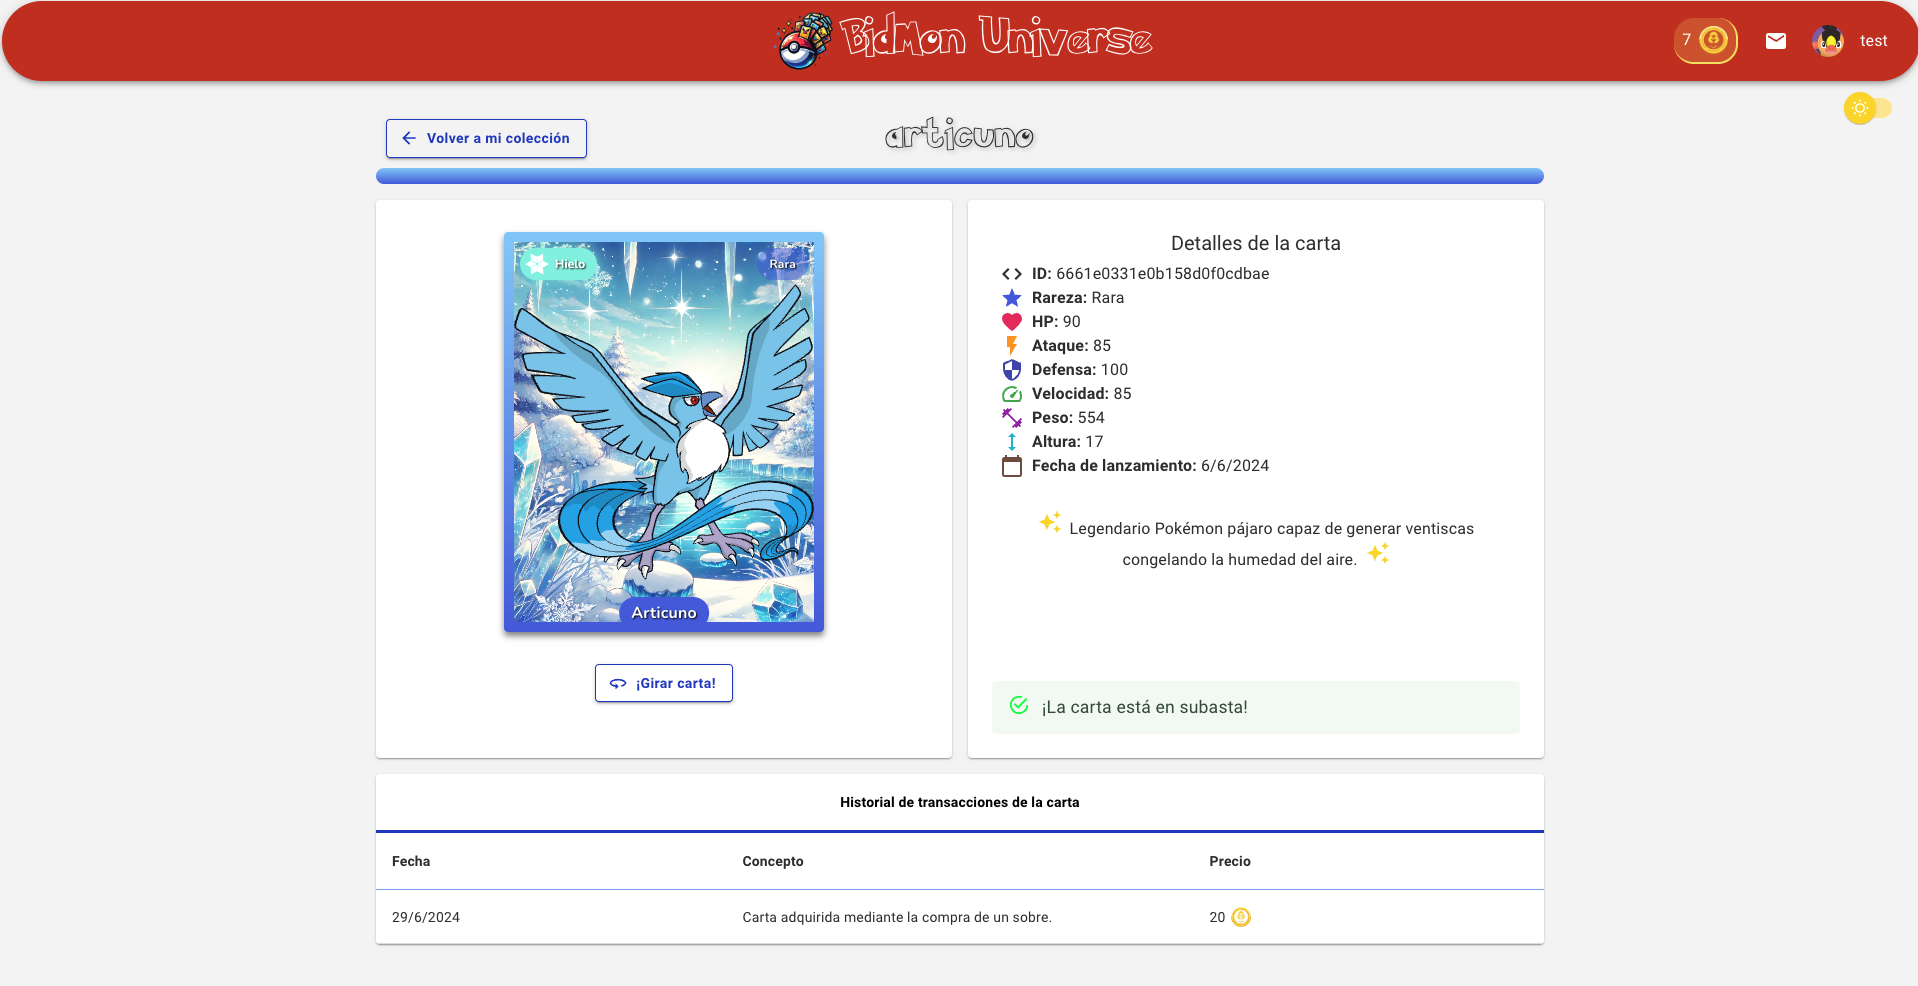
\includegraphics[width=0.8\textwidth]{figures/6-Analisis/6-Interfaz/interfaz/subasta_creada2.png}
    \caption{Alerta de que la carta está en subasta.}
    \label{fig:interfaz-subasta-alerta}
\end{figure}

Si el usuario cancelase en algún momento el proceso de subasta, se cerraría el modal.


\subsubsection{Compra de un sobre de cartas}
El proceso de compra de un sobre de cartas es más sencillo que el de la subasta de una carta.
El usuario pulsa el botón de \textit{Comprar sobre} del sobre que desea comprar y se le abrirá un modal de confirmación.

\begin{figure}[H]
    \centering
    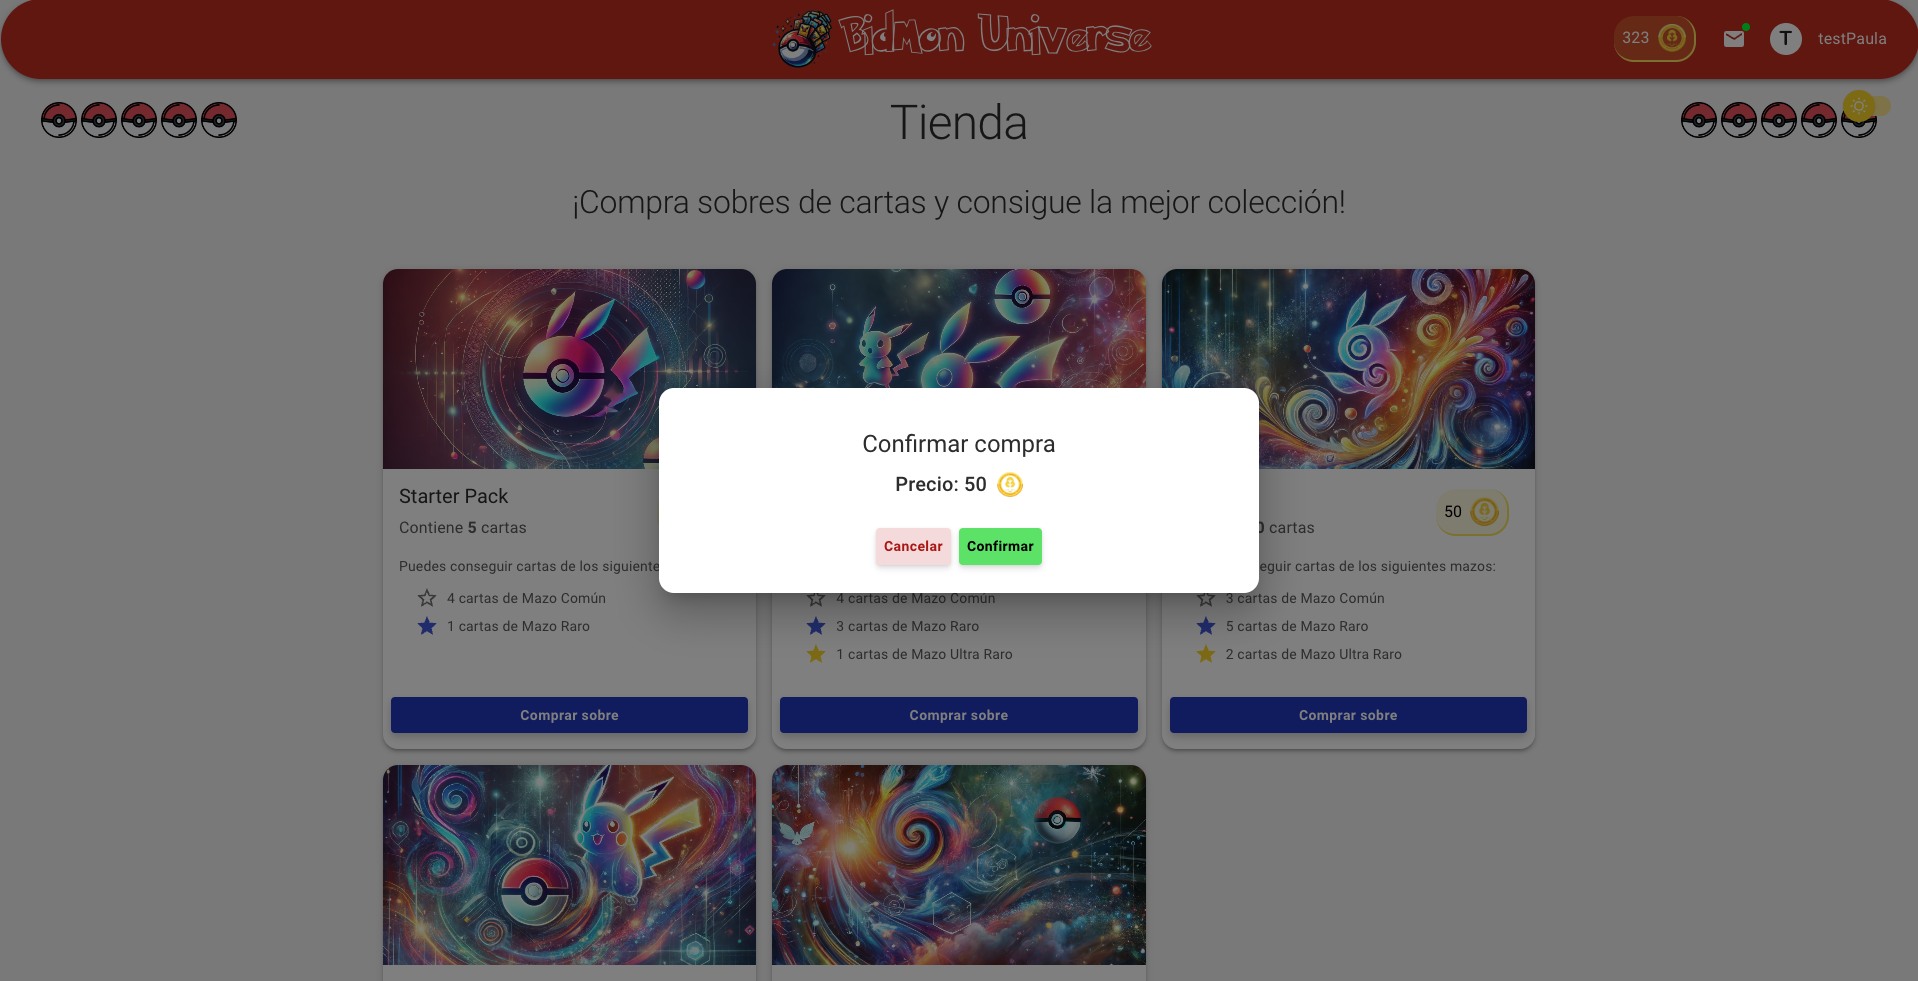
\includegraphics[width=0.8\textwidth]{figures/6-Analisis/6-Interfaz/interfaz/compra_sobre1.png}
    \caption{Modal de confirmación de compra de sobre.}
    \label{fig:interfaz-compra-sobre}
\end{figure}

Una vez que el usuario confirma la compra, se le mostrarán las cartas que ha obtenido en el sobre y un mensaje de éxito.
Estas cartas aparecen volteadas por lo que el usuario debe pulsar sobre ellas para verlas.
Tiene la opción de cerrar el modal o de ir a la colección de cartas para ver las cartas que ha obtenido.

\begin{figure}[H]
    \centering
    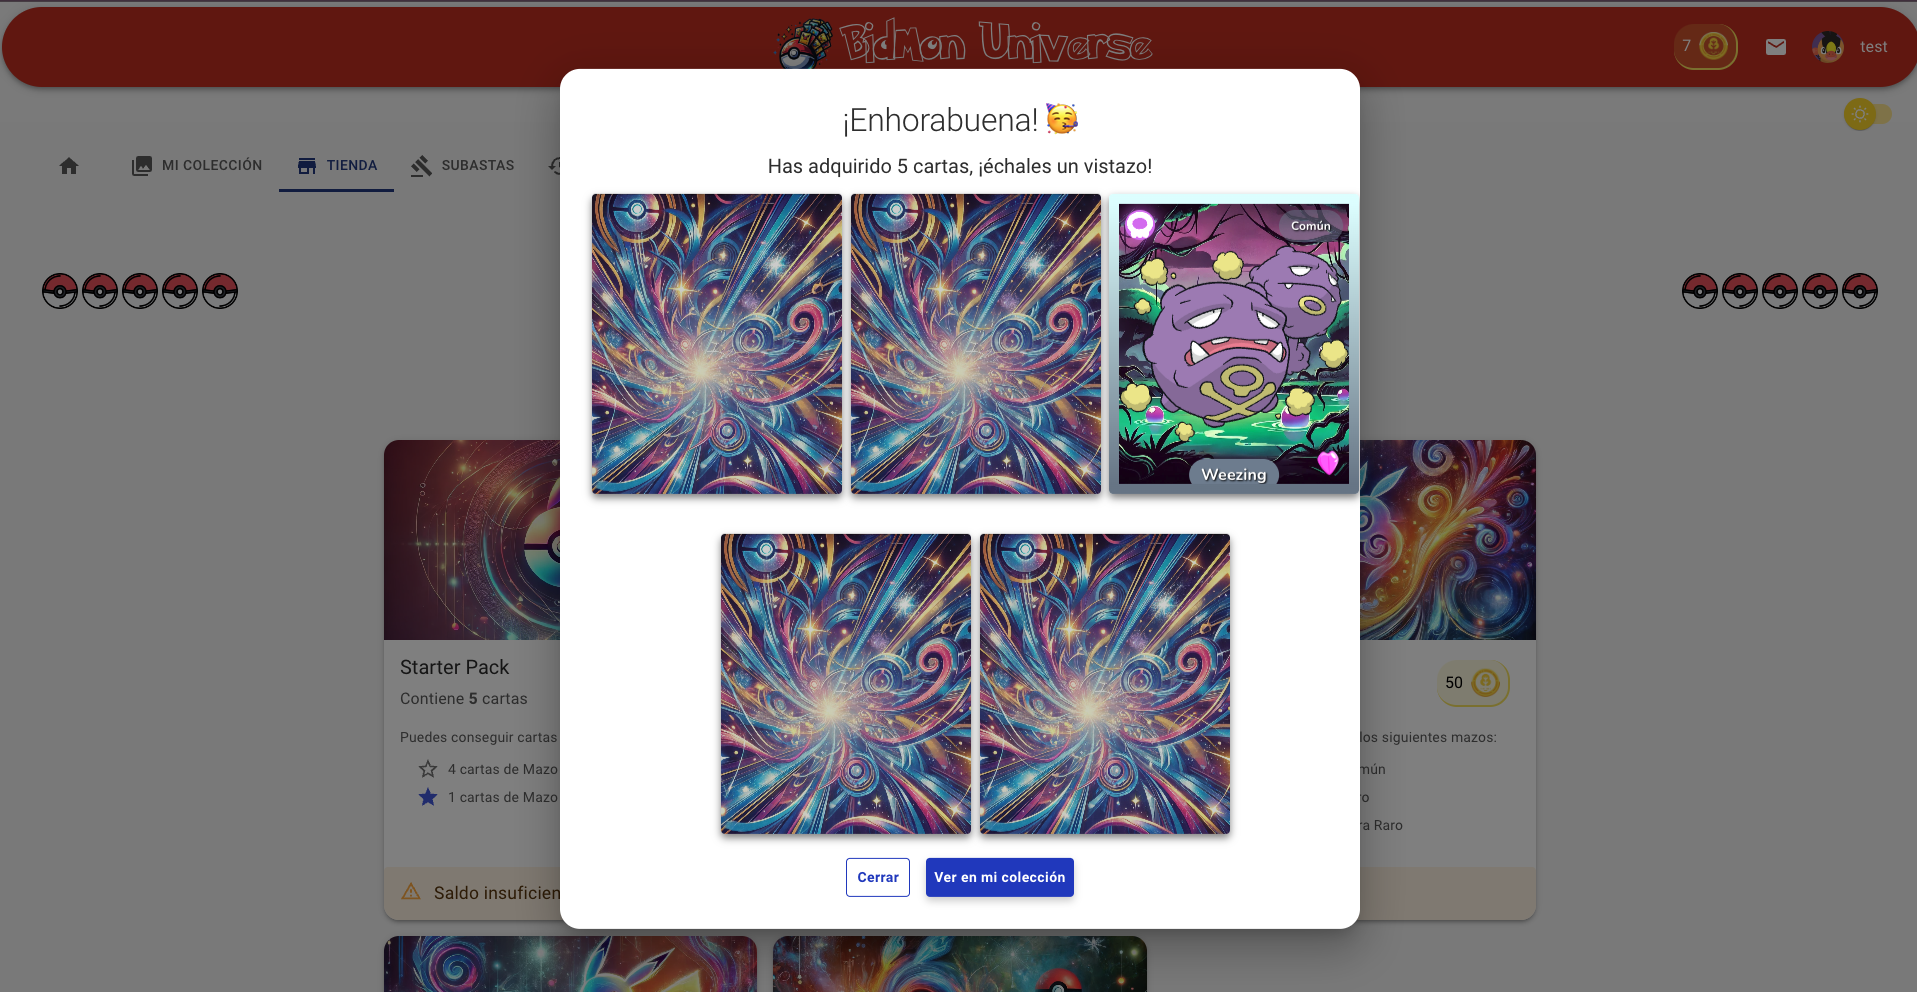
\includegraphics[width=0.8\textwidth]{figures/6-Analisis/6-Interfaz/interfaz/compra_sobre.png}
    \caption{Modal de cartas obtenidas en el sobre.}
    \label{fig:interfaz-sobre-comprado}
\end{figure}


